\defChapterTarget[ArchitecturalDesign]{Architectural design}
    \section{\textit{Overview}: High-level components and their interaction}
    The whole software that will become the main core of the SafeStreets
    initiative will be developed as a distributed application, which means that
    the software will be executed (or run) on multiple devices within a network.
    It will have a three-layers logic and be divided as following:
    \begin{itemize}
        \item \textbf{P}: The \textbf{\emph{presentation}} layer will handle all
        \textit{incoming} (\textit{and outcoming}) relations with the customers
        \item \textbf{A}: The \textbf{\emph{application}} layer will work as a
        "man in the middle" between the \textbf{P}resentation layer and the
        \textbf{D}atabase layer and will hold all the needed logic for the
        software to correctly work;
        \item \textbf{D}: The \textbf{\emph{database}} layer will be needed in
        order to store and manage all needed (and requested) information of the
        initiative;
    \end{itemize}
    Each and every one of the layers the architecture will be composed by a
    (group of) machines. By doing this, it is meant to provide, to each layer,
    its own dedicated hardware, for either scalability, failure handling and
    flexibility reasons.\\
    The following image shows the high-level architecture of the system without
    providing any detail of the components which will form the structure of the
    software itself, which will be tackled later in this document.

    \begin{figure}[H]
        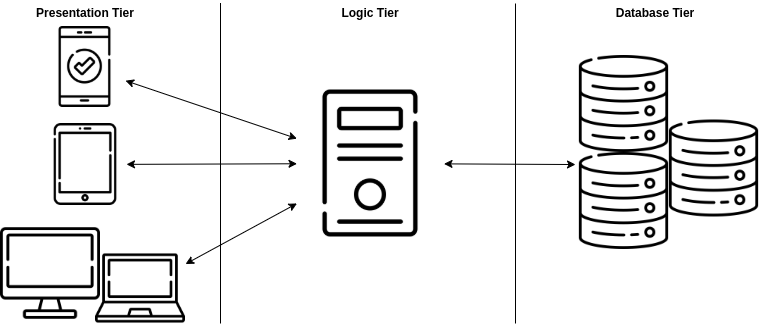
\includegraphics[scale=0.45]{dd/resources/images/HighLevelStructure.png}
        \caption{High-level architecture}        
    \end{figure}
 
    The introduction of the \textbf{P}resentation layer has been considered in
    order to allow a thin client architecture and let less performing devices
    access SafeStreets initiative and give a smoother feeling when using either
    the mobile or web version of the software. By doing so, this allows also for
    an high reusability of the code, since the logic is all implemented in the
    single \textbf{A}pplication layer, which allows different devices to access
    the same logic. The latter is the only tier which deals with two other tiers
    at the same time and is in charge of accessing data from the
    \textbf{D}atabase layer and pass it to the clients back and forth. In
    addition, the \emph{man in the middle} communicates with the Data tier
    synchronously when it comes to access the needed data, but asynchronously
    when storing and writing actions are required.\\
    \\
    The software will exploit a \textbf{P}latform \textbf{a}s \textbf{a}
    \textbf{S}ervice (\textbf{\emph{PaaS}}) provided by
    Amazon\textsuperscript{\textcopyright}. It has been chosen to create a
    \textbf{V}\textbf{P}\textbf{C} in order to attend the requirements stated in
    section 3.5 \emph{"Software System Attributes"} of the RASD. This will help
    also to augment the system scalability and improve the perfomances, as well
    as the reliability and security of the information stored in the system. \\
    The system is going to be modeled on a \emph{scale out} architecture: this
    will be improve the performance, as well as the failure management, by
    replicating nodes. This kind of architecture has been chosen, instead of a
    scale up architecture, as the latter is not suitable for a system thatplans
    to be eventually expanded and furtherly serve more and more customers. It
    comes without saying that the chosen kind of architecture will require the
    implementation of a \emph{load-balancing system} as well as a
    \emph{\textbf{S}hared \textbf{D}isk \textbf{C}onfiguration} (\textbf{SDC})
    in order to let all hardware write and read the same information at any
    moment. The latter has been chosen over a Shared Memory Configuration as it
    provides a certain degree of fault tolerance and does not create a
    bottleneck on the memory bus.\\
    Furthermore, in order to comply to the correct chain of custody that the
    system requires and to protect all sensible information of all customers,
    the installation of a proper \textbf{D}e\textbf{M}ilitarized \textbf{Z}one
    (\textbf{\emph{DMZ}}) is needed. This is accomplished by a series of
    firewalls created around the core tier of the software, the
    \emph{Application Tier}, the one that, if compromised by malicious users,
    could provide access to both other layers.\\ 
    \\ 
    The following image shows a detailed representation of the concepts above
    explained. Thanks to the decision of exploiting
    Amazon\textsuperscript{\textcopyright}'s services and its VPC, all the above
    mentioned architectural characteristics are automatically implemented, as
    the whole service is customizable and easily implementable.

    \begin{figure}[H]
        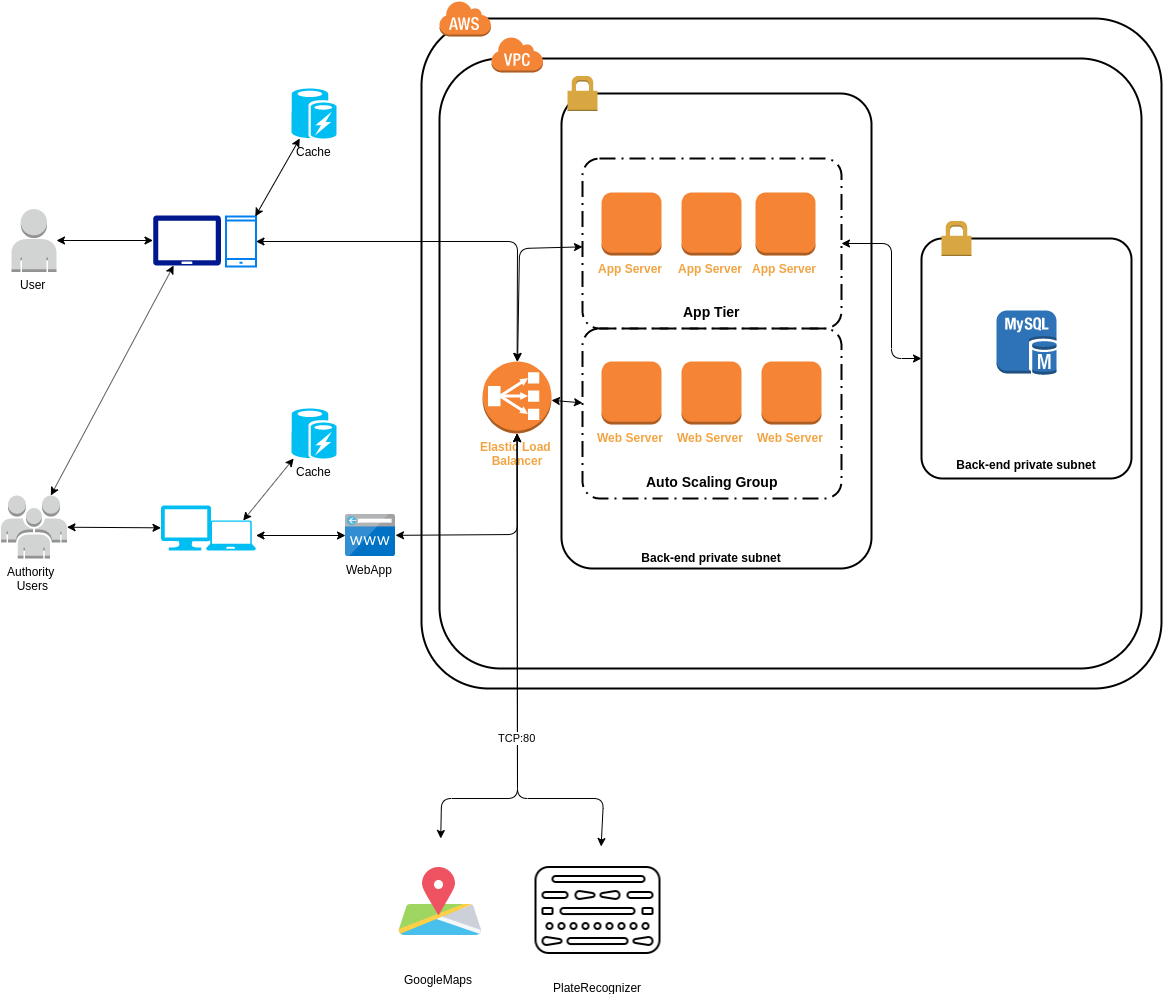
\includegraphics[scale=0.3]{dd/resources/images/ArchitecturalStructure.png}
        \caption{Architectural structure} 
    \end{figure}

    It is easily noticeable that there is no mention of the photo forensic
    software (\emph{Ghiro, per instance}) as this general architecture focuses
    on the software itself. Any additional photo forensic software, like the one
    proposed, has to be considered part of the "package" sold, but not needed to
    be developed as an already functioning software has been chosen. The sole
    purpose of SafeStreets is to ensure that the program is actually used and
    allow an automatic redirection to it. 

    \section{Component view}
    \begin{figure}[H]
        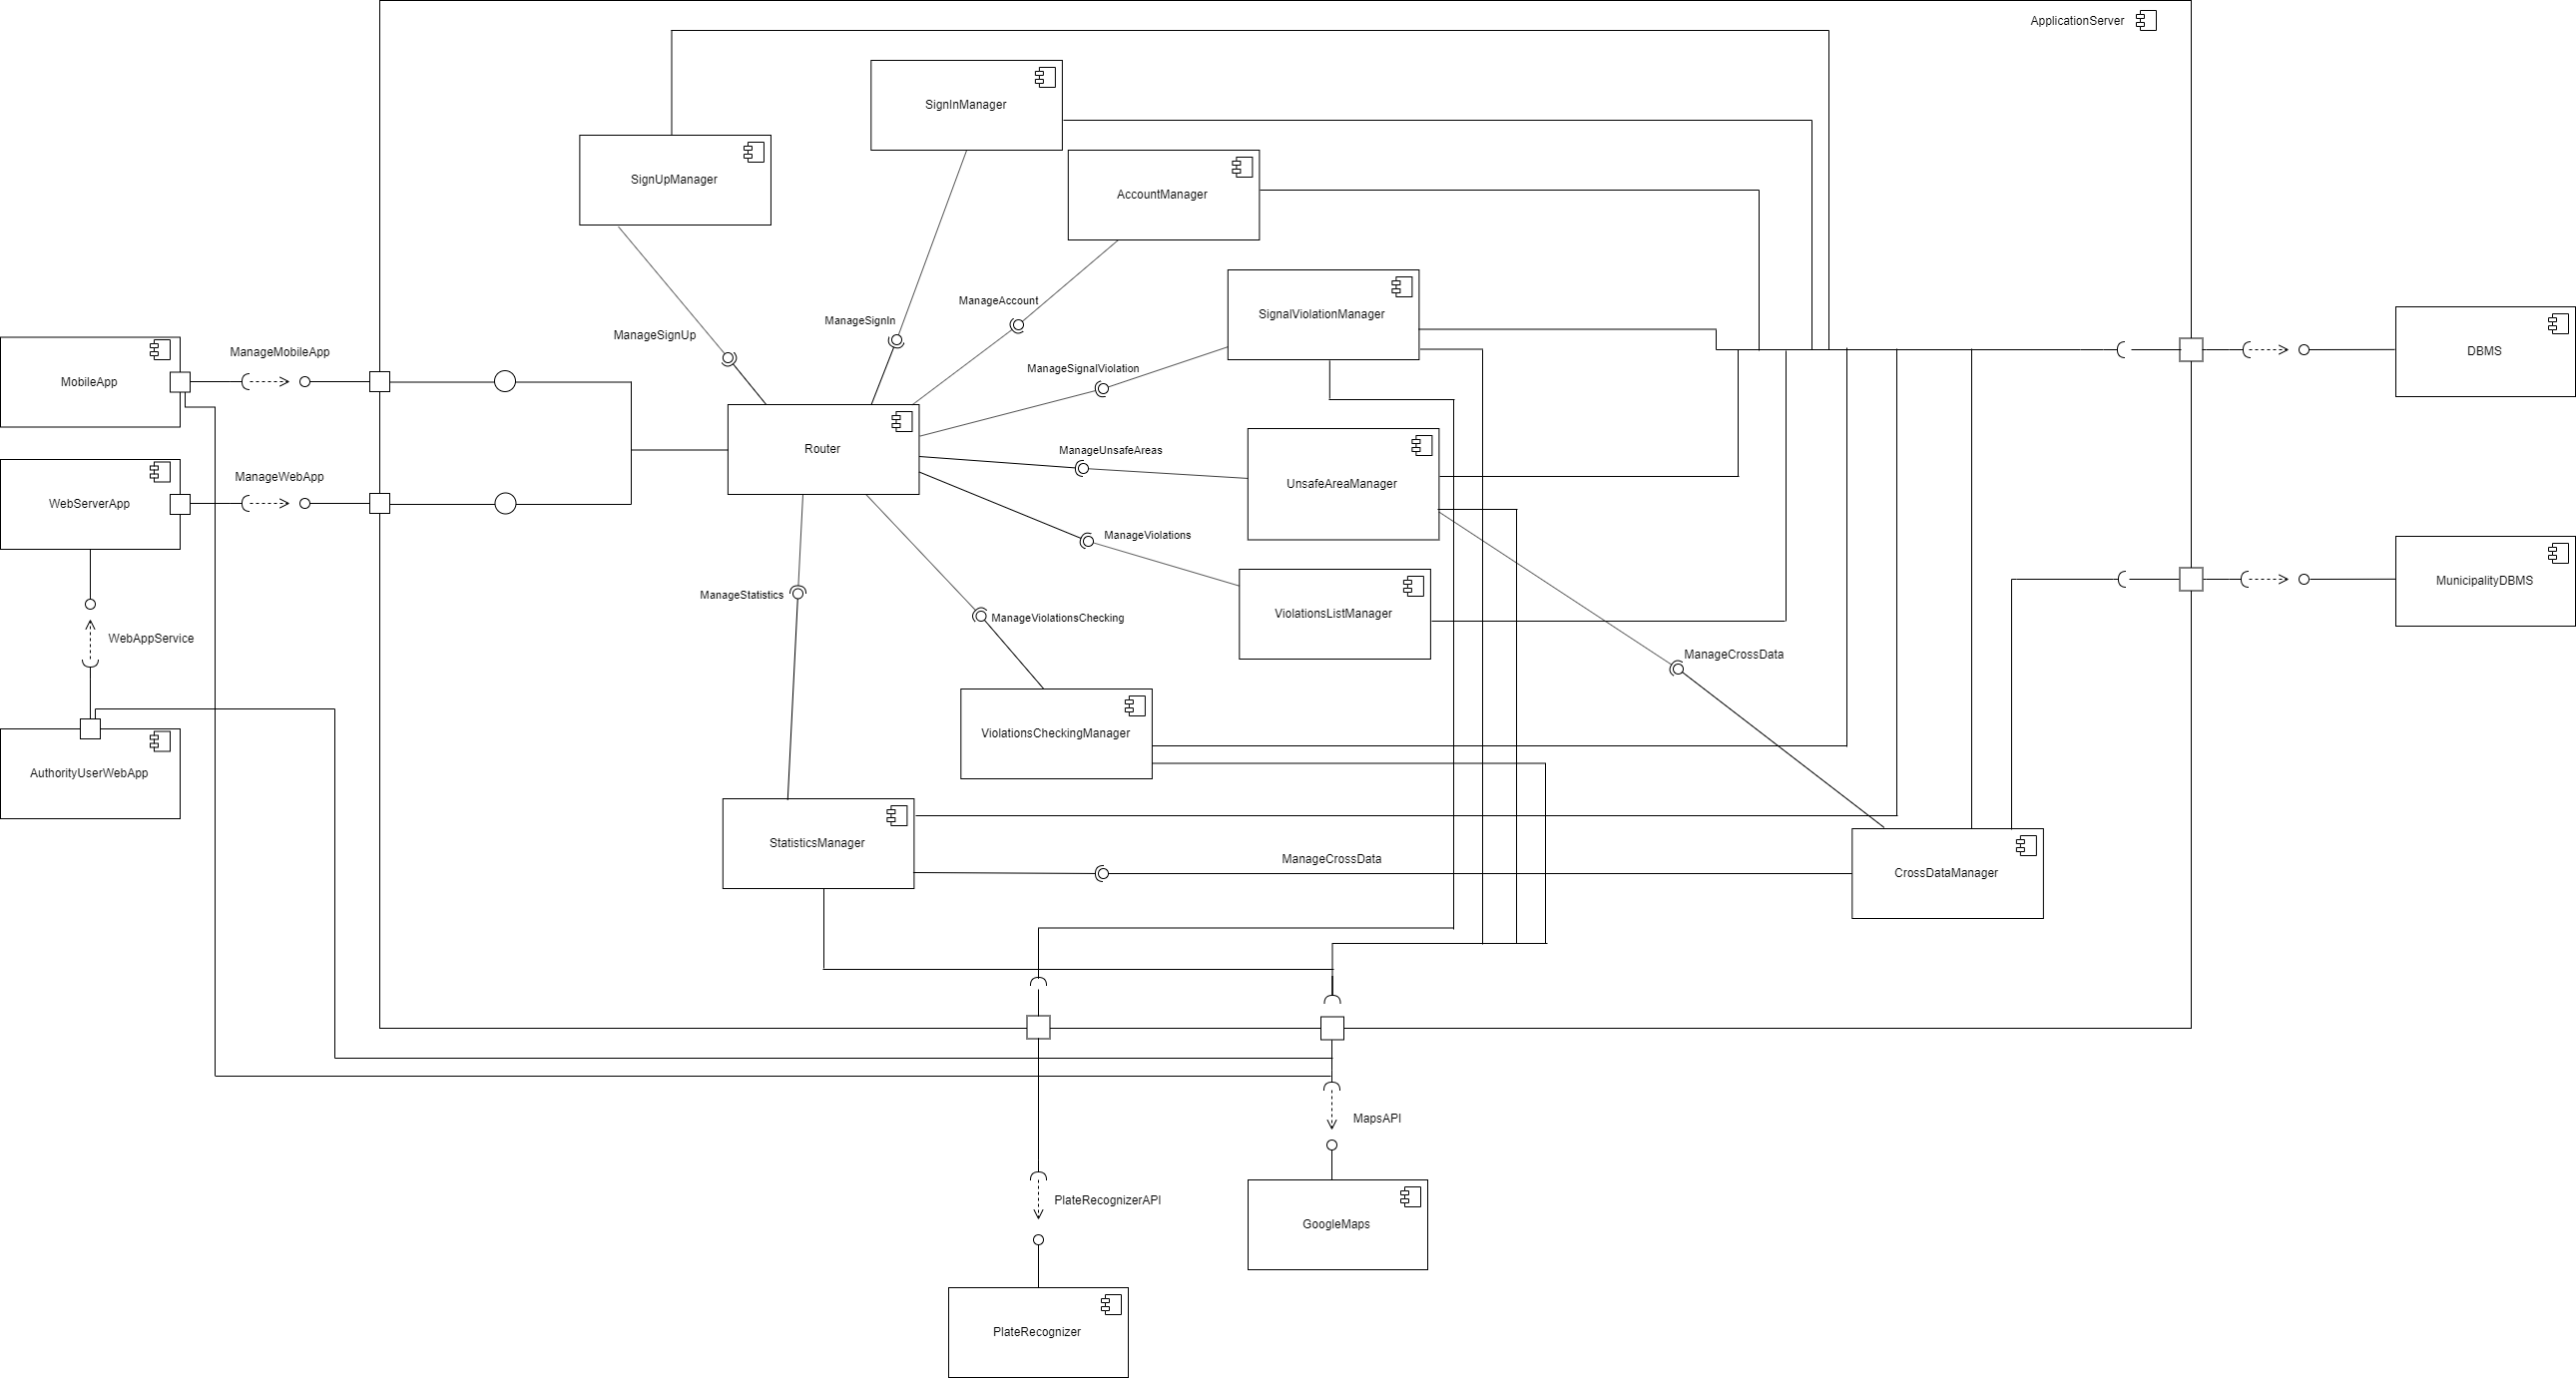
\includegraphics[scale=0.19,angle=90]{dd/resources/images/ComponentDiagram.png}
        \caption{Component Diagram}        
    \end{figure}
    \begin{itemize}
        \item \textbf{Router}:it manages messages and function calls coming from
        other subsystems in order to pass the data to the correct element of the
        system. It eventually calls the correspondent method/function on it.
        Furthermore, the router is partitioned according to the type of the
        interacting components because of the different functionalities. 
        \item \textbf{SignUpManager}: this component provides all the procedures
        to allow customers to register to SafeStreets. Obviously, this
        components has also to interact with SafeStreets DBMS to store the
        registration data and to run a check about the chosen email, password
        and AuthoritiesID or fiscal code.
        \item \textbf{SignInManager}: it contains all the logic devoted to the
        authentication of the customers. It check the authentication parameters
        using the data stored on SafeStreets DBMS.
        \item \textbf{AccountManager}: this component provides all the
        procedures to manage the account and interacts with SafeStreets
        DBMS.
        \item \textbf{SignalViolationManager}: it deals with the signalations of
        violations made by the users. It interacts with SafeStreets DBMS.
        \item \textbf{UnsafeAreasManager}: this component provides all the users
        the possibility to see the unsafe areas. It receives all the information
        from SafeStreets DBMS and municipality DBMS through CrossDataManager. 
        \item \textbf{ViolationsListManager}: with this component the user can
        see all the violations he/she has reported. The authority user can see
        all the violations reported in his/her area. It interacts with SafeStreets DBMS.
        \item \textbf{ViolationsCheckingManager}: this component provides the
        authority user the ability to check che violations. It interacts with SafeStreets DBMS.
        \item \textbf{StatisticsManager}: this component provides the authority
        user the possibility to see all the statistic generated crossing the
        data on violations. It receives all the information
        from SafeStreets DBMS and municipality DBMS through CrossDataManager. 
        \item \textbf{CrossDataManager}: it crosses data from SafeStreets
        DBMS and from the municipality DBSM to generate the statistics
        and the unsafe areas.
    \end{itemize}    
    \newpage

    \begin{figure}[H]
        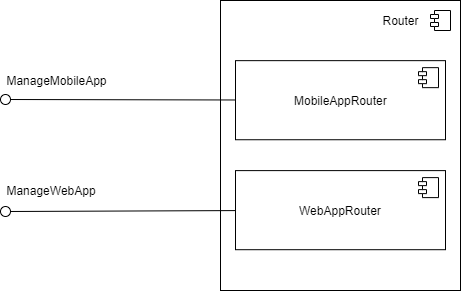
\includegraphics[scale=0.8]{dd/resources/images/RouterComponents.png}
        \caption{Detailed view of router components}        
    \end{figure}
    \newpage
    \section{Deployment view}
    The following image is a deployment diagram which represents the
    architecture of the system as distribution(deployment) of software artifacts
    to deployment targets(node). Artifacts represents elements obtained with a
    development process. Nodes can represent either hardware or software
    environments.
    \begin{figure}[H]
        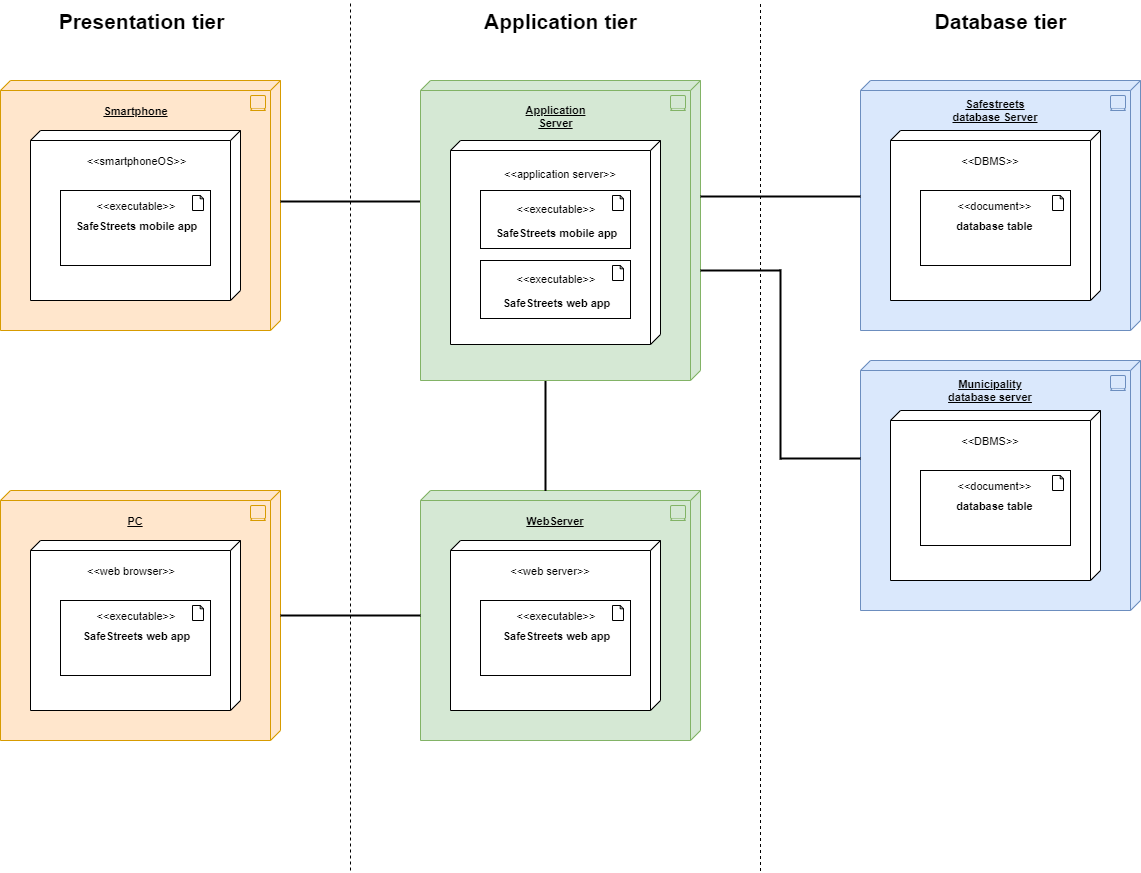
\includegraphics[scale=0.35]{dd/resources/images/DeploymentDiagram.png}
        \caption{Deployment view}        
    \end{figure}
    The three tiers contain:
    \begin{itemize}
        \item \textbf{Presentation tier}: in this tier the presentation logic is
        deployed. Users are provided with a mobile application on their mobile
        devices and authority users are provide with both a mobile application
        and a web application accessible from a common browser. The mobile
        application must be developed for most of the devices (both iOS and
        Android version). Both user and authority user ask to communicate to the
        application server in order to retrieve data, signal a violation, check
        violations or unsafe areas.
        \newpage
        \item \textbf{Application tier}: in this thier the application logic is
        deployed. The application server allows the mobile application and the
        web application to access data stored into the SafeStreets database. The
        application server also implements the business logic and handles the
        requests. The mobile application directly addresses the application
        server. The web server allow authority users to use SafeStreets
        services. If it can't provide some information it forwards the requests
        to the application server.
        \item \textbf{Database tier}: in this tier data access must be deployed.
        The internal Safestreets' database is going to be a relational database
        (which is going to be furtherly explained in this document). In the
        meantime, the software is going to require an exclusive access to third
        party databases (eg. municipality databases), which are going to expose
        a series of API calls in order to retrieve relative data on certain
        areas of said municipality, traffic violations and so on.
    \end{itemize} 
    \newpage   
    \section{Run-time view}
        \subsection{Signal a violation}
        \begin{figure}[H]
            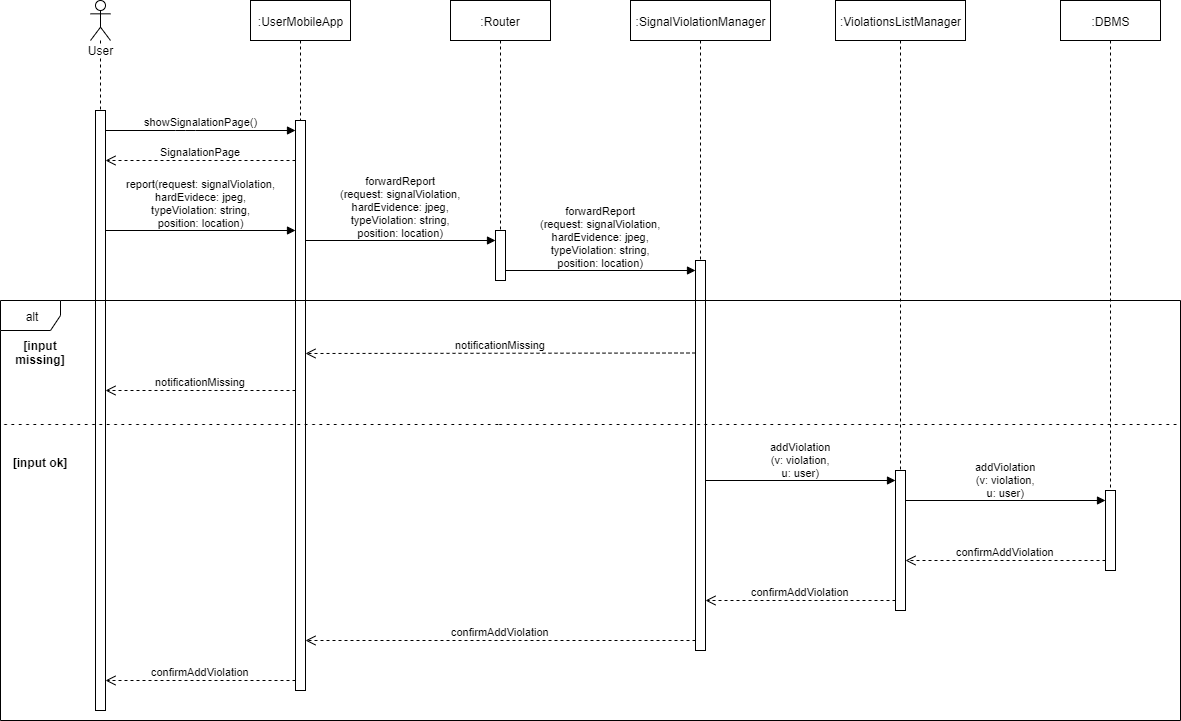
\includegraphics[scale=0.35]{dd/resources/images/RuntimeView-SignalViolation}
            \caption{Runtime View - Signal a violation}        
        \end{figure}
        In this sequence diagram the process through which a user, already
        logged in, can signal a violation to the authorities is shown. Once the
        web app has rendered the page to report a violation, the user can insert
        all the needed input data to perform the action (the position, photos of
        hard evidence, type of violation are here thought to be contained in the
        request object. The position is assumed to be entered by the user
        manually, the detection of the online location by Google Maps is
        neglected). When submitted, the request is sent to the Router, which
        forwards it to the right component, i.e. the 'SignalViolationManager'.
        The latter is responsible for checking the input inserted by the user:
        if there are some missing or invalid input, an error message is sent
        back to the user who can recompile the form and resubmit the new data.
        Otherwise, if all the inputs are valid, the request with all data of the
        violation and the parameter user set to the user who have done the
        report is sent to 'ViolationListsManager', which forwards it to the DBMS
        (which adds it to the list of reports of that municipality). At this
        point, the DBMS send the confirm of the operation to the components up
        to the user who it's ready to send other reports or to return to his
        menu.

        \subsection{SignUp and SignIn}
        \begin{figure}[H]
            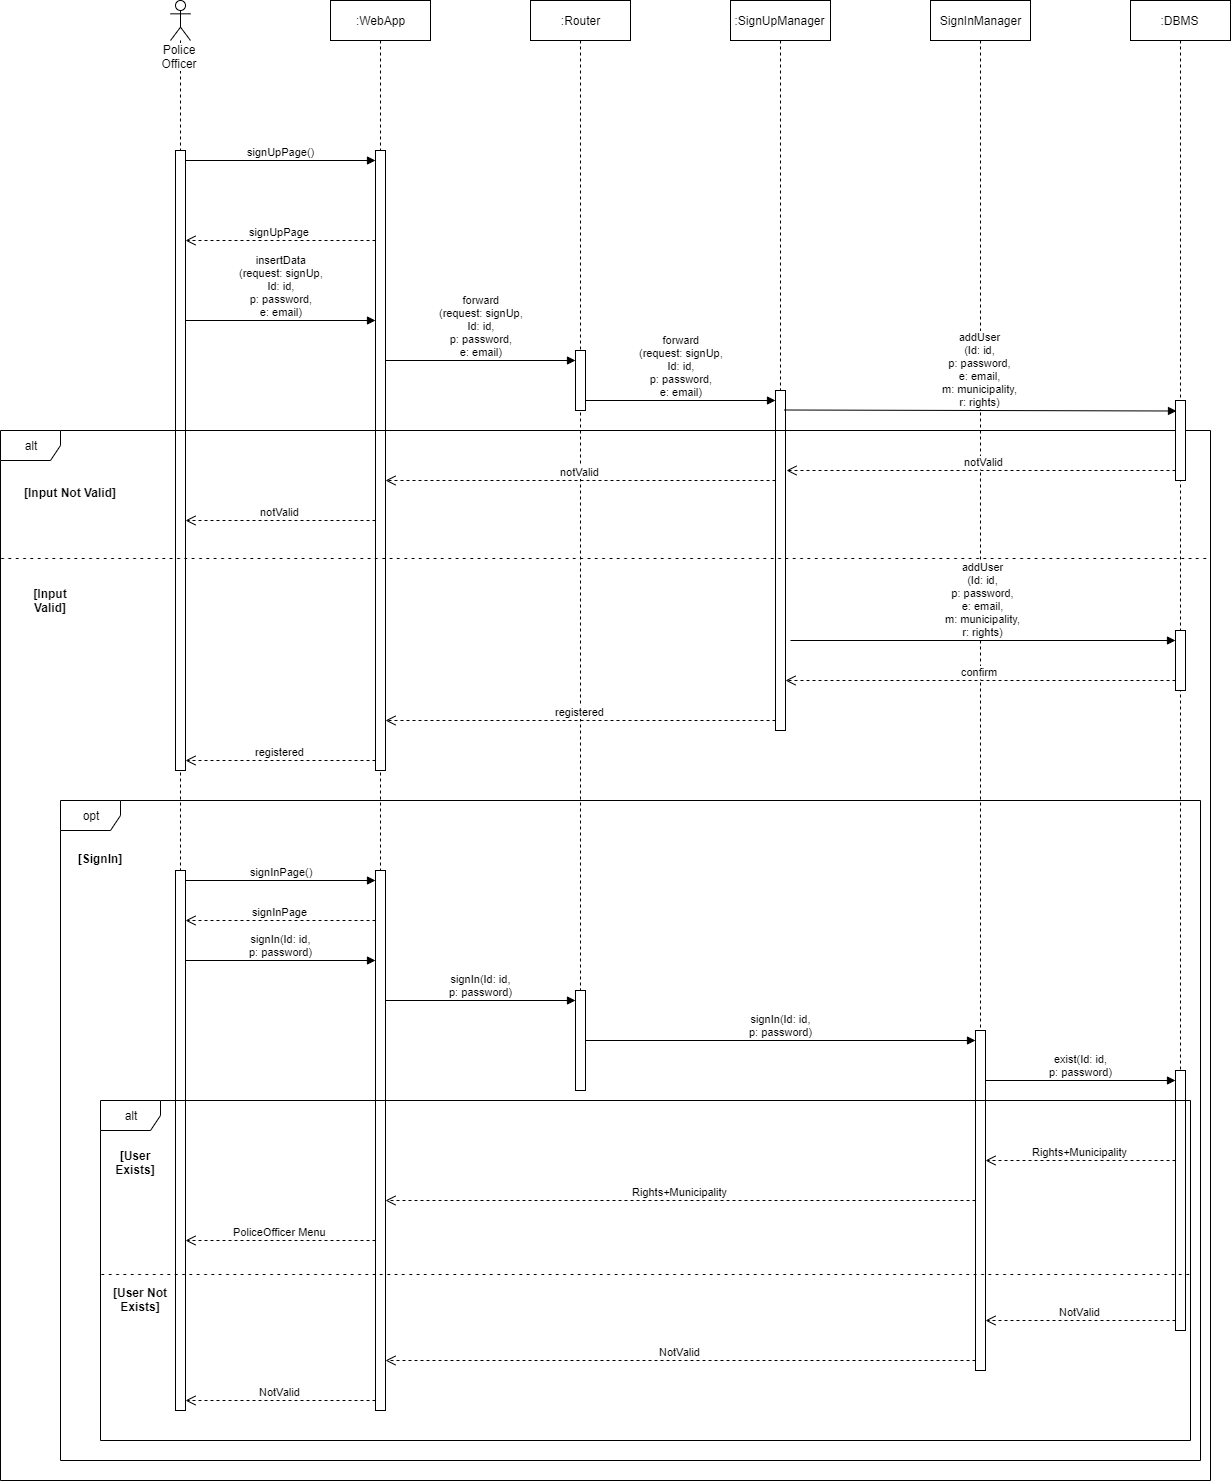
\includegraphics[scale=0.35]{dd/resources/images/RuntimeView-SignUp+SignIn}
            \caption{Runtime View - SignUp and SignIn}        
        \end{figure}
        In this sequence diagram the process of sign up and subsequently sign in
        is shown. Once the WebApp has rendered the page to signup, the Police
        Officer insert his data (AuthorityId, email, password). When submitted,
        the request is sent to the Router, which forwards it to the right
        component, i.e. the 'SignUpManager'. The latter is responsible for
        checking the input inserted by the Police Officer: if there are some
        missing or invalid input or the Authority results already registered, an
        error message is sent back to the user. Otherwise, if all the inputs are
        valid, SignUpManager analyze the AuthorityId and understand the
        municipality of competence of the Police Officer and his rights, so it
        adds the parameters of municipality and rights to the other data and
        send them to the DBMS which add a new AuthorityUser. At this point, the
        DBMS send the confirm of the operation to the components up to the user
        who can, if he want, sign in to the service. He therefore, once the
        WebApp has rendered the page to signin, inserts his Id and password.
        When submitted, the request is sent to the Router, which forwards it to
        the right component, i.e. the 'SignInManager'. The latter is responsible
        for checking the input and asks to the DBMS if there exists a couple
        <Id,password> into the database. If there no exists, SignInManager send
        an error to the user, otherwise, once understand the right of the user
        (i.e. PoliceOfficerRights) and his municipality, he send these data to
        the WebApp which shows the personal menu to the Police Officer. 

        \subsection{Analyze Unsafe Areas}
        \begin{figure}[H]
            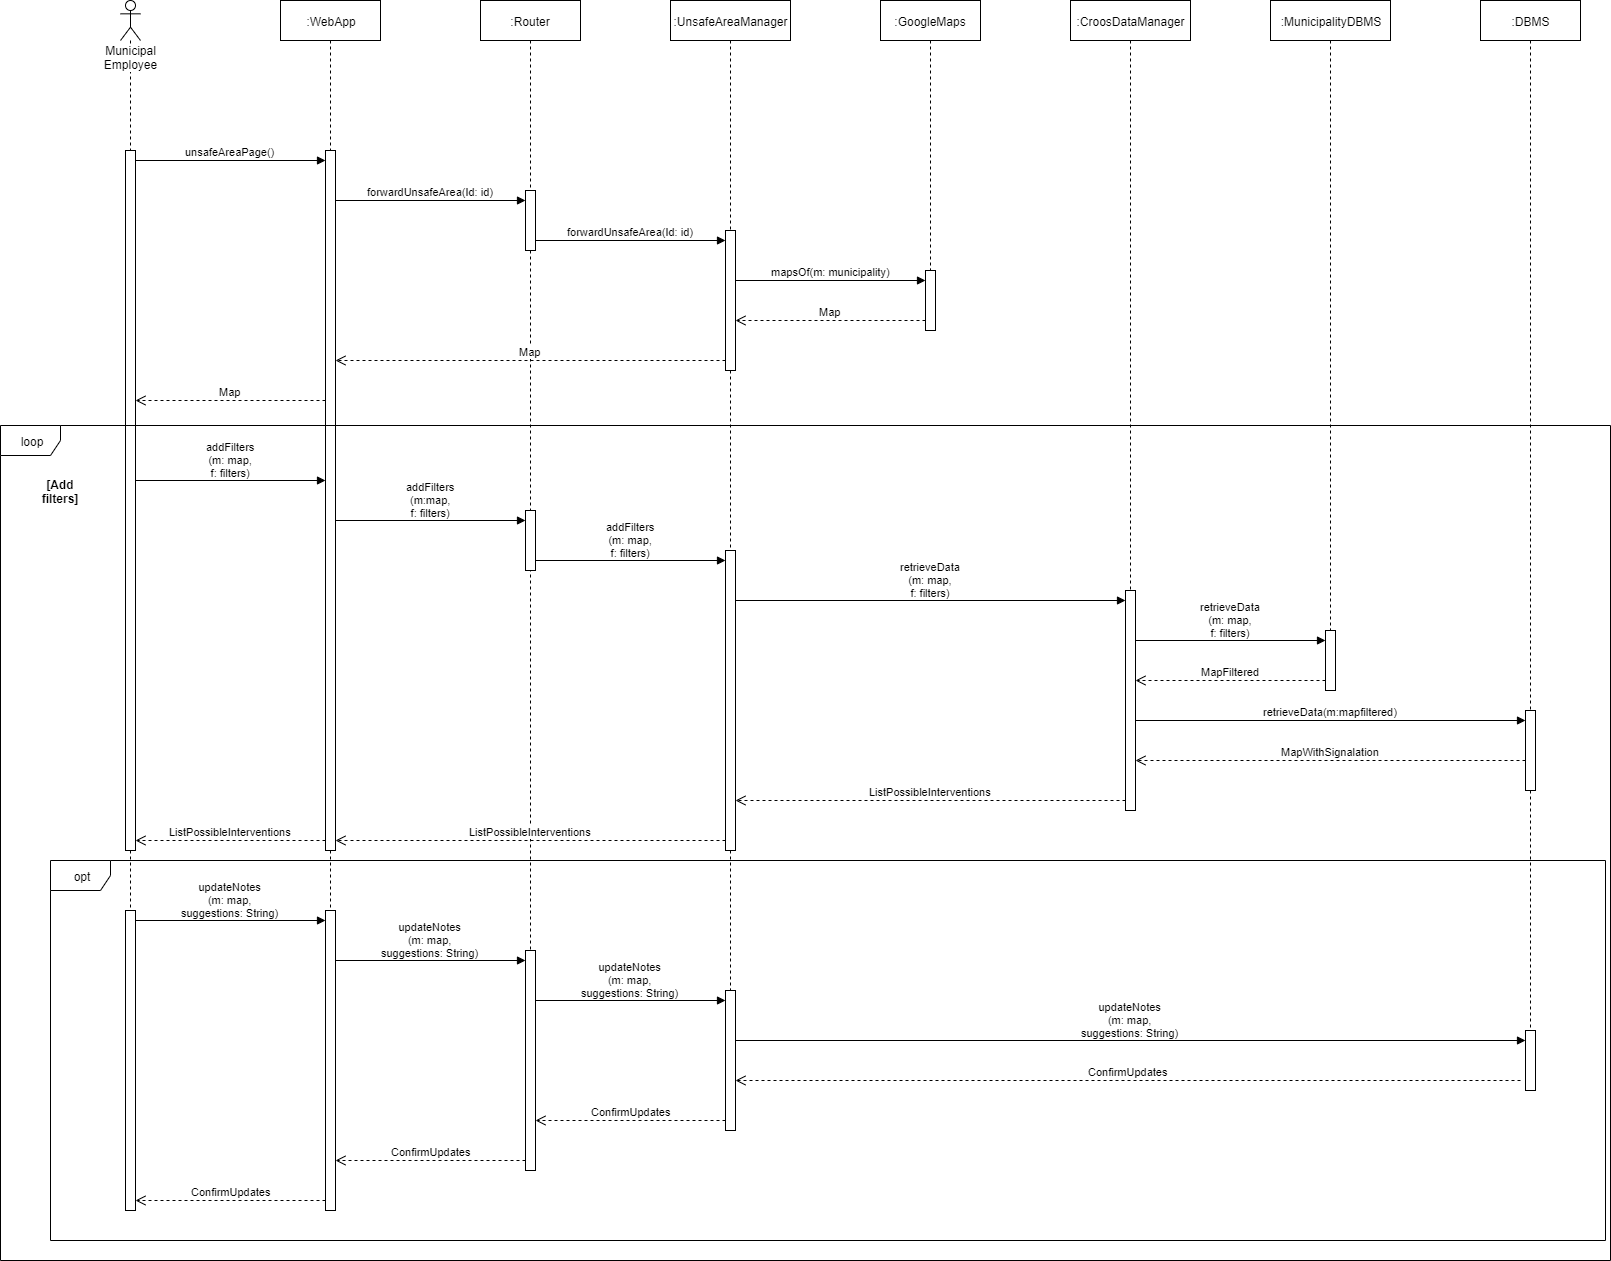
\includegraphics[scale=0.28]{dd/resources/images/RuntimeView-UnsafeAreas}
            \caption{Runtime View - Unsafe Areas}        
        \end{figure}
        In this sequence diagram the process of analyze the Unsafe Areas is
        shown. The Municipal Employee request the UnsafeAreaPage to the WebApp
        which forwards the request to the Router adding the Id of the municipal
        employee. The Routher forwards it to the right component, i.e. the
        'UnsafeAreaManager'. The latter understand, through the Id, the
        municipality of competence of the Municipal Employee and asks the map to
        Google Maps. Therefore the map of the municipality is sent up to the
        employee. At this point, the employee can add filters to his maps and,
        through the same chain, UnsafeAreaManager receives the map from Google
        Maps and forwards it and the filters to CrossDataManager. The latter
        forwards all the data to the Municipality Database which responds with
        the map filtered. Moreover the CrossDataManager forwards all the data to
        the DBMS of SafeStreets which responds with the map and signalation. Now
        CrossDataManager has all the data that it needs to cross the data and he
        sends the resulting map up to the employee. The employee can decide to
        update or delete or add suggestions and he send them to
        UnsafeAreaManager which forwards them to the DBMS of Safestreets, the
        process ends with the confirm of the DBMS sent up to the employee.

        \subsection{Statistics}
        \begin{figure}[H]
            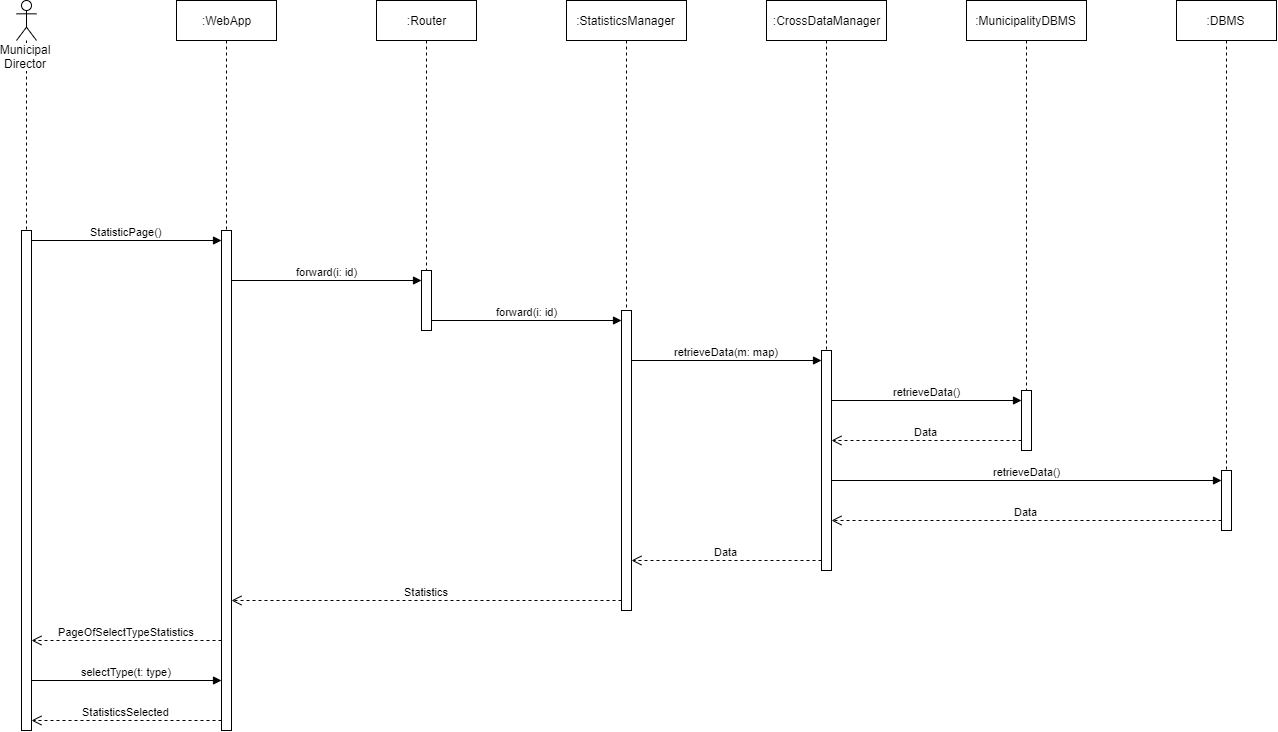
\includegraphics[scale=0.34]{dd/resources/images/RuntimeView-Statistics}
            \caption{Runtime View - Statistics}
        \end{figure}
        In this sequence diagram the process of analyze the Statistics is shown. 
        The Municipal Director request the StatisticsPage to the WebApp which forwards 
        the request to rhe Router adding the Id of the municipal director. The Router 
        forwards it to right component, i.e. the 'StatisticsManager'. The latter 
        understand, through the Id, the municipality of competence of the Municipal 
        Director and forward the request to the CrossDataManager. The latter retrieve 
        the data from the municipality and from the DBMS of SafeStreets. Now CrossDataManager 
        has all the data that it needs to cross the data and he sends the resulting data up 
        to the employee. The employee can decide which type of statistics to select and the 
        process enda with the WebApp that show to the director the statistics selected.

    \newpage
    \section{Component interfaces}
    \begin{figure}[H]
        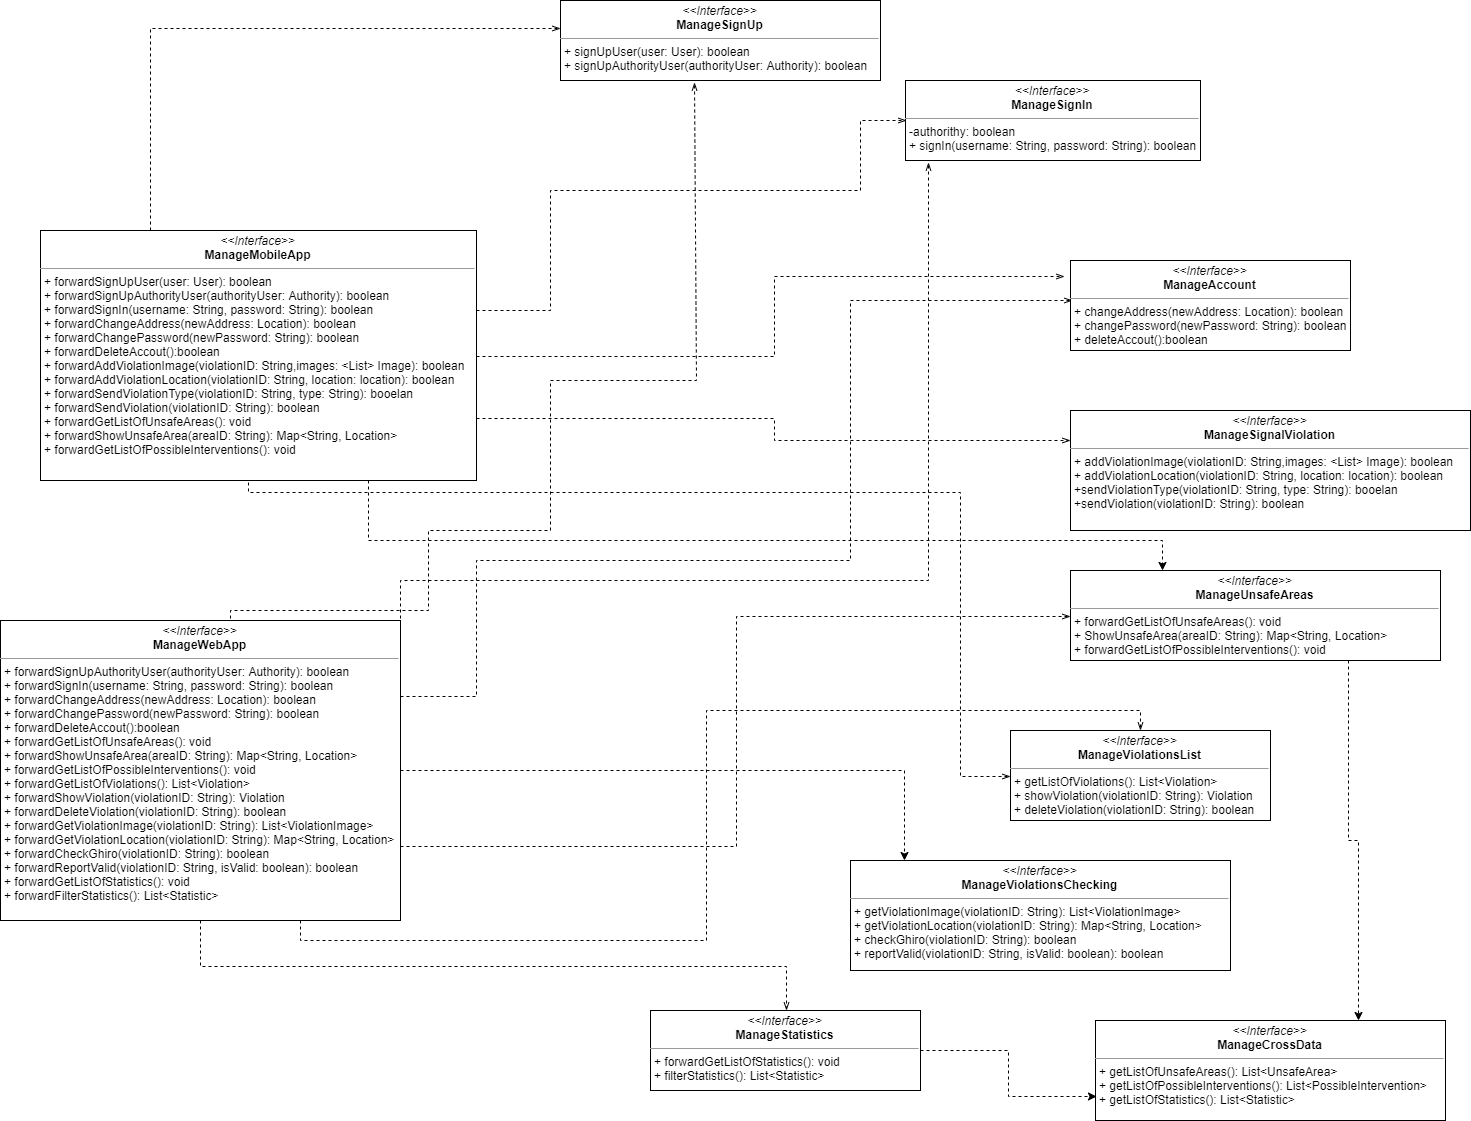
\includegraphics[scale = 0.331, angle=90]{dd/resources/images/ComponentInterfaces.png}
        \caption{Component Interfaces} 
    \end{figure}
    The above picture shows an ideal representation of how the main component
    interfaces, which main functions they should be implementing and how they
    should be communicating with each other.\\
    The first thing that jumps to the eye is the existence of the two biggest
    interfaces: \emph{ManageMobileApp} and \emph{ManageWebApp}. Both of them
    will work as connectors by taking input from the customers and forward them
    the actual logic tier which processes those inputs and returns the correct
    outputs, which are once again forwarded by these two components to the UI.\\
    
    Furthermore, the \emph{ManageCrossData} component is worth of mention as it
    is a critical point for the correct functioning of two main parts of the
    SafeStreets initiative. This component manages all interactions that are
    going to happen with third party databases and the information they hold,
    cross reference it with the SafeStreets' acquired info and redirects the
    output to either the \emph{ManageUnsafeAreas} or \emph{ManageStatistics}
    components. 

    \newpage
    \section{Selected architectural styles and patterns}  
        \subsection{Architectural styles}
    
            \subsubsection{RESTful architecture}
            It has been decided to use a RESTful architecture in order to
            develop SafeStreets website. REST architectural style allows
            requesting systems to access and manipulate web resources by using a
            uniform and predefined set of rules. REST is very useful in systems
            like SafeStreets where there are different clients who request
            resources and a server which provides the resources. In a RESTful
            architecture we must satisfy some different constraints:
            \begin{itemize}
                \item \textbf{Uniform Interface}: there exists a uniform way to
                interact with SafeStreets server regardless user's device or
                application.
                \item \textbf{Stateless}: the client hanldes the state for the
                request and the server doesn't store anything related to the
                session. This constraint allows simple server design.
                \item \textbf{Cacheable}: this constraint accellerates
                client-server communications because it completely eliminates
                some interations.
                \item \textbf{Client-server}: client doesn't know anything about
                the business logic and server doesn't know anything aboyt the
                client. and it's UI. In SafeStreets system authority users uses
                a web app that communicates with the web server which in turns
                communicates with the application server where is located the
                business logic.
                \item \textbf{Layered system}: an application architecture with
                multiple layers allows the presence of a lot of multiple servers
                between the client and the end server. The architecture is then
                more flexible and secure because each layer doesn't know
                anything about any layer other than that of immediate layer.
                \item \textbf{Code on demand}: is an optional feature and it
                isn't used in SafeStreets system.
            \end{itemize}    

            \subsubsection{Three tier architecture}
            The architecture of SafeStreets is multilayered, composed of three tiers:
            \begin{itemize}
                \item \textbf{Presentation layer}: is used to present the data in a way
                that the user can understand. It enables the usage of the services
                offered to the user. The presentation layer of the the users is the
                smartphone and for authority users are both the smartphone and the
                browser.
                \item \textbf{Application layer}: is used to coordinate the application.
                It receives and computes the requests send by the presentation layer and
                it also interacts with the database.
                \item \textbf{Database layer}: stores the information provided by the
                application layer. The information is also passed back to the
                application tier for processing.
            \end{itemize}    
            Three tier architecture is very useful because it allows to change or
            upgrade one of the three tiers without any problem and so it makes the
            system more flexible and reusable. Furthermore it makes the system safer
            because it separates the access to data from the other layers.
                

        \subsection{Design Patterns}
            \subsubsection*{Model View Controller (MVC)}
            \begin{figure}[H]
                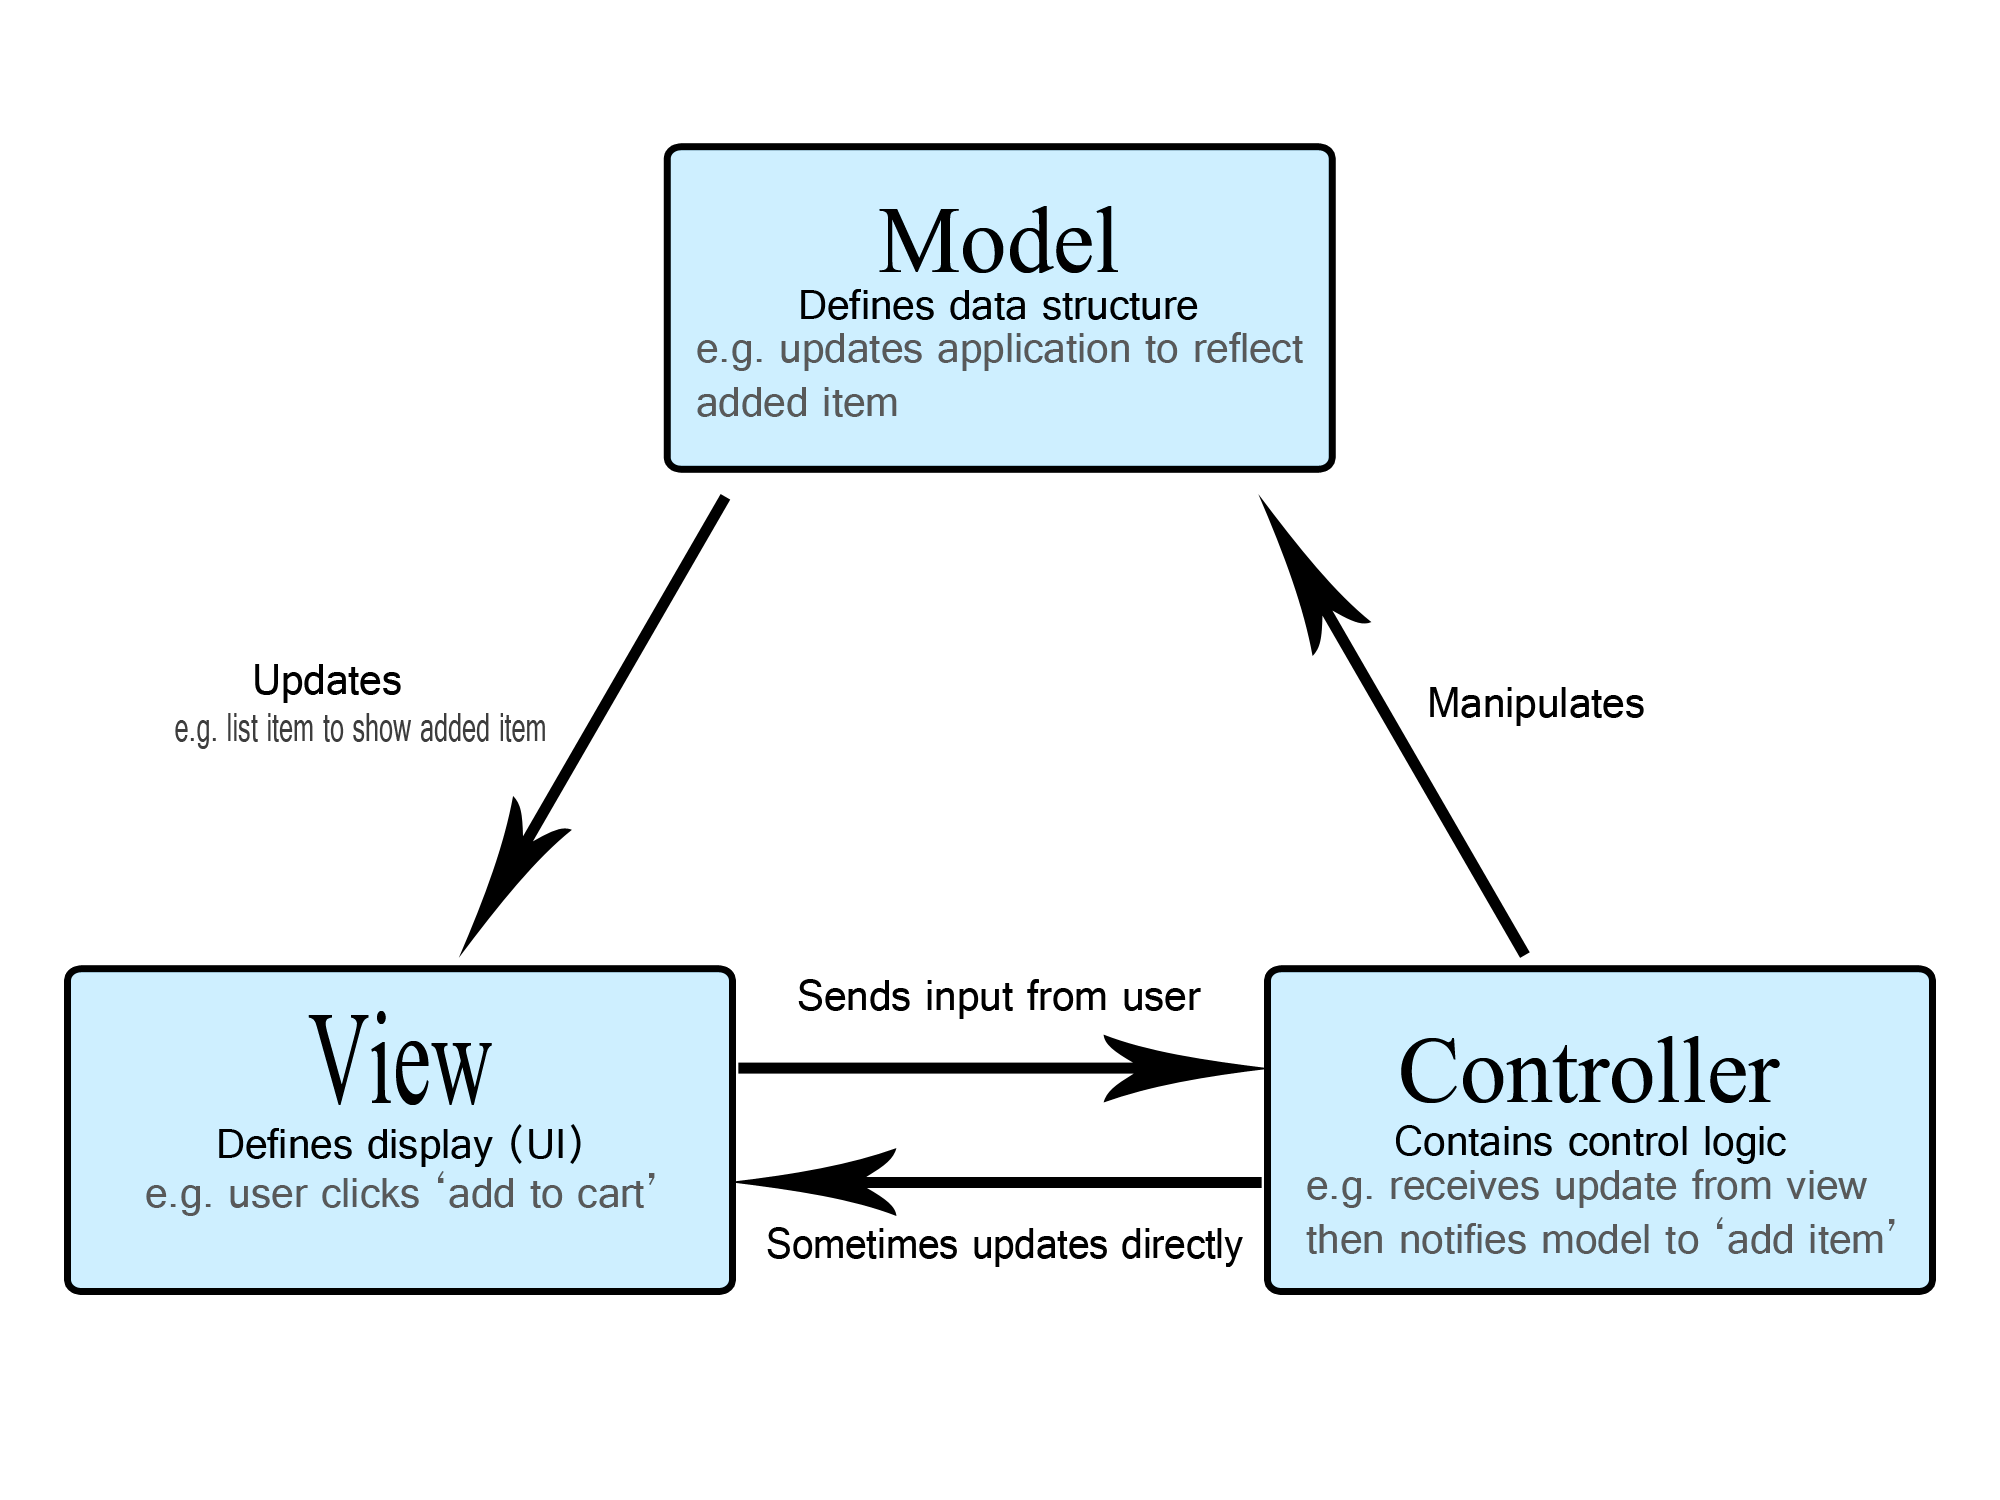
\includegraphics[scale=0.9]{dd/resources/images/MVC.png}
                \caption{Model view controller}        
            \end{figure}
            Model view controller is a very useful and quoted design pattern.
            MVC is used to separate the fundamental parts of the application and
            in particular it  emphasizes a separation between the software’s
            business logic and display. The three parts of Model View Controller
            design pattern are:
            \begin{itemize}
                \item \textbf{Model}: manages all the data and the business
                logic
                \item \textbf{View}: handles the GUI used by all the users
                \item \textbf{Controller}: acts on both model and view, it
                routes commands to the view and model elements  
            \end{itemize}    
            MVC is also very useful because the decoupling of these three
            components allows parallel development and code reuse.
    \section{Other design decisions}
    \subsection{Virtual Private Cloud}
    It has been chosen to exploit the services of
    Amazon\textsuperscript{\textcopyright} in order to simplify the process of
    creation and future modification of the architecture, in case any of the
    constraints should be needed to adapt to the constantly changing market's
    requirements. \emph{Amazon\textsuperscript{\textcopyright} VPC} is the
    networking layer for Amazon\textsuperscript{\textcopyright} \textbf{EC2}
    (\textbf{A}mazon\textsuperscript{\textcopyright} \textbf{E}lastic
    \textbf{C}ompute \textbf{C}loud), which provides scalable computing capacity
    on the \textbf{A}mazon\textsuperscript{\textcopyright} \textbf{W}eb
    \textbf{S}ervices cloud (\textbf{AWS}). This service provides a series of
    features as, for example, the ones important to SafeStreets' initiative:
    \begin{itemize}
        \item Virtual computing environments (\emph{or instances});
        \item Various configurations of CPU, memory, storage and networking
        capacity (\emph{instance types});
        \item Firewalls that enable developers to specify protocols, ports and
        source IP ranges that can reach the \emph{instances} using
        \emph{security groups};
        \item Static IPv4 addresses for dynamic cloud computing, known as
        Elastic IP addresses. This is used in case of failure of an instance by
        rapidly remapping the failed address to another existing instance;
    \end{itemize}

    \subsection{Thin Client}
    In a "Thin Client" architecture the server does most of the work while the
    client is lightweight. In this architecture the client is designed to be
    online all the time and to communicate with a server. If network connection
    is down the application of course doesn't work, but we don't need to
    implement any offline modules because the core idea of the application is
    comunication itself. Furthermore thin client architecture allows the
    application to keep all the real business logic protected on the server.
    \\Google Maps APIs could be considered an exception to this paradigm because
    are used directly by the client.

    \subsection{Relational Database}
    Relational databases are the most common type of digital databases. The
    model is based on relations between data and it is solid, avoids duplication
    of data and enables developers to work with safe and predictable results. By
    building the relational model, the data are organized into one (or more)
    tables (or \emph{relations}) of columns and rows, with a unique key
    identifying each row (or \emph{tuples}) which can be linked between to each
    other. By doing so, this model allows to handle higly structured data and
    provides support for ACID transactions. The structure is very flexible and
    it can be scaled up without problems because adding data without modifying
    the existing ones is simple. In addition relational databases use very
    expressive and mature query languages such as SQL and the whole management
    of the database is left to handle to the DBMS (\textbf{D}ata\textbf{B}ase
    \textbf{M}anagement \textbf{S}ystem).
     